\documentclass[11pt]{article}

% --- packages (kept to a widely-available core so the paper compiles with
%     pdflatex / tectonic / latexmk without extra installs) ---
\usepackage[utf8]{inputenc}
\usepackage[T1]{fontenc}
\usepackage[margin=1in]{geometry}
\usepackage{amsmath,amssymb}
\usepackage{graphicx}
\usepackage{booktabs}
\usepackage{xcolor}
\usepackage{caption}
\usepackage[hidelinks]{hyperref}

\graphicspath{{figures/}}

% labels for the integrity convention used throughout
\newcommand{\meas}{\textcolor{black}{\textsc{[m]}}}      % MEASURED
\newcommand{\expd}{\textcolor{gray}{\textsc{[e]}}}       % EXPECTED
\newcommand{\code}[1]{\texttt{#1}}

\title{\textbf{Steering Microbial Communities with an Energy-Based JEPA
World Model}\\[2pt]
\large Inverse Dynamics, Metric Geometry, and the Limits of Planning in Latent Space}

\author{Belgacem Ben Ziada\\
\small École Polytechnique\\
\small \texttt{BBenziada@gmail.com}}

\date{}

\begin{document}
\maketitle

\begin{abstract}
We study energy-based Joint-Embedding Predictive Architectures (JEPA) as
\emph{world models of living systems under intervention}: given the state of a
microbial community and an applied perturbation (a dose on a candidate-species
panel), predict the next state \emph{entirely in latent space}, never
reconstructing abundances. Building on the \texttt{eb\_jepa} framework, we
contribute (i) a permutation-invariant set-transformer encoder that consumes a
community as an unordered set of species tokens; (ii) a generalized
Lotka--Volterra (gLV) ``Two-Rooms'' simulator whose cyclic inter-guild
competition makes target states reachable only through \emph{non-monotonic}
intervention sequences; and (iii) an action-conditioned latent world model with
an inverse-dynamics (IDM) auxiliary. Across controlled, seed-replicated
experiments we report a mix of positive, negative, and diagnostic results, all
measured. (1)~In a collapse-prone regularization regime, the IDM term rescues
the decodability of the applied intervention from the latent state
($R^2{:}~0.520\!\rightarrow\!0.748$, $+0.229$, positive in all three seeds),
a textbook slow-feature collapse-and-recovery; the effect is regime-dependent
and shrinks under strong variance regularization. (2)~On a MDSINE2-style
hold-one-subject-out temporal benchmark the JEPA world model is the strongest
forecaster at every horizon. (3)~On a real infant-gut downstream task a frozen
JEPA embedding with a SIGReg (LeJEPA) regularizer matches or beats a published
baseline. (4)~Planning is a \emph{diagnosed negative and its closure}: a
pure-JEPA latent is faithful for one-step prediction yet is \emph{not a metric
space}, so latent model-predictive control succeeds $0\%$ of the time across
eight independent levers; supplying a single isometry auxiliary turns planning
$0\%\!\rightarrow\!100\%$ at oracle quality (final distance $0.804$ vs.\ oracle
$0.790$), and this closure generalizes to $4/4$ held-out gLV instances.
(5)~Removing sequencing-technology nuisance is hard: an adversary (DANN) fails
while a deterministic moment-matching alignment (CORAL) gives a partial,
linear-only fix. We close with a real-world generality check on Tahoe-100M drug
perturbations. Our central lesson: \emph{faithful one-step prediction does not
imply a plannable metric}, and the metric must be supplied, not merely hoped
for.
\end{abstract}

\noindent\textbf{Reproducibility \& integrity.} Every quantity below is labelled
\meas\ \textsc{measured} (from a committed run, with job/figure provenance) or
\expd\ \textsc{expected} (a hypothesis or literature value). Negative and
surprising results are reported as-is. The single load-bearing integrity
correction (an unseeded-decoder fluke) is documented in
Section~\ref{sec:integrity}. Code, configs, result JSONs, and the figures
reproduced here live in \code{examples/microbiome\_jepa/},
\code{examples/microbiome\_benchmark/}, and \code{examples/tahoe\_probe/}; a
complete quantitative log is in \code{docs/WORK\_REPORT.md}.

\section{Introduction}

Microbial communities --- the gut, soil, water --- are high-dimensional dynamical
systems we increasingly wish to \emph{control}: nudge a dysbiotic gut toward a
healthy configuration, design a probiotic intervention, or screen a drug's
effect on a cell. Control requires a \emph{world model}: a map from
$(\text{state},\text{action})$ to the next state. We ask whether the
Joint-Embedding Predictive Architecture (JEPA) family~\cite{lecun2022path}
--- which predicts in a learned representation space rather than input space,
under an energy/anti-collapse objective --- yields world models that are good
enough not just to \emph{predict} a community's trajectory but to \emph{plan}
interventions on it.

JEPA is attractive here for two reasons. First, microbial state is
compositional, sparse, and permutation-invariant (a community is a \emph{set}
of species, not an ordered vector); predicting in latent space sidesteps the
pathologies of reconstructing zero-inflated counts. Second, a learned latent
provides a natural substrate for energy-based planning: descend the predicted
energy landscape toward a target embedding. But JEPA also has a well-known
failure mode --- it preferentially encodes \emph{slow} features and can collapse
away the fast, action-driven signal we most need for control~\cite{sobal2022}.

This paper is an honest, exhaustive study of where this works and where it does
not. We build the necessary machinery (a set encoder, a controllable simulator,
an action-conditioned predictor with an inverse-dynamics term), establish
positive results on representation quality and short-horizon forecasting, and
then confront planning head-on. The planning story is the heart of the paper: a
pure-JEPA latent that is demonstrably faithful for one-step prediction
nonetheless fails completely as a \emph{planning metric}, and we trace the
bottleneck layer by layer to the geometry of the representation --- then close
the loop with a single, well-understood auxiliary.

\paragraph{Contributions.}
\begin{itemize}
\item A permutation-invariant \textbf{set-transformer encoder} for microbial
communities that plugs into \texttt{eb\_jepa}'s temporal predictor and
regularizers unchanged (Section~\ref{sec:encoder}).
\item A \textbf{gLV ``Two-Rooms'' simulator} with cyclic, rock-paper-scissors
inter-guild competition, giving provably non-monotonic reachability --- a clean,
controllable testbed for planning (Section~\ref{sec:glv}).
\item A measured \textbf{IDM collapse-and-recovery} result: the inverse-dynamics
auxiliary restores fast (action) decodability in the collapse-prone regime, and
the effect is regime-dependent (Section~\ref{sec:idm}).
\item A \textbf{layered diagnosis of planning} (controllability $\to$
representation geometry $\to$ readout fidelity) showing that
\emph{faithful prediction $\neq$ plannable metric}, and a \textbf{metric
(isometry) auxiliary} that closes the planning loop $0\%\!\rightarrow\!100\%$
and generalizes across instances (Section~\ref{sec:planning}).
\item Studies of \textbf{anti-collapse regularizers} (VICReg vs.\ SIGReg/LeJEPA)
and of \textbf{sequencing-technology invariance} (adversarial vs.\
moment-matching), plus a real-world generality check on \textbf{Tahoe-100M}
drug perturbations (Sections~\ref{sec:sigreg}--\ref{sec:tahoe}).
\end{itemize}

\section{Background and Related Work}

\paragraph{JEPA and energy-based SSL.} JEPA~\cite{lecun2022path} predicts the
representation of a target from a context, scoring candidates by an energy
$\mathcal{E}(x,x')=\lVert g_\phi(f_\theta(x)) - f_\theta(x')\rVert^2$. To avoid
the trivial constant solution, an anti-collapse regularizer is added; we use
VICReg's variance--covariance terms~\cite{bardes2022vicreg} and, as an
alternative, the SIGReg isotropy objective of LeJEPA~\cite{lejepa2025}, an
Epps--Pulley characteristic-function test that pushes the embedding toward an
isotropic Gaussian. A world model is the action-conditioned case: the predictor
$g_\phi(f_\theta(x), q_\omega(a))$ takes an encoded action $a$.

\paragraph{Slow-feature collapse.} Sobal et al.~\cite{sobal2022} show that a temporal JEPA
trained only to predict the next latent tends to encode \emph{slow} features
(trajectory identity/basin) and discard the \emph{fast} signal (the applied
action). The standard remedy is an inverse-dynamics model (IDM): require that
the action be recoverable from consecutive latents, forcing the encoder to keep
fast information. This is the mechanism we test directly in
Section~\ref{sec:idm}.

\paragraph{Microbiome dynamics and planning.} Generalized Lotka--Volterra (gLV)
models are the workhorse of microbial ecology; MDSINE2~\cite{mdsine2} formalizes
inference and hold-one-subject-out forecasting on real time series. For control
we use model-predictive path integral (MPPI) control~\cite{williams2017mppi},
sampling action sequences and reweighting by a cost. Our nuisance-removal study
draws on domain-adversarial training (DANN)~\cite{ganin2015dann} and deep
moment-matching (CORAL)~\cite{sun2016coral}. The closest learned-representation
neighbour for cellular perturbations is GeneJEPA~\cite{genejepa2025}; we compare
our own baselines cleanly rather than claiming to beat its protocol.

\section{Methods}

\subsection{Problem setup}
A community state at time $t$ is a set $\{s_i\}$ of present species, each with an
embedding and a log-abundance; the action $a_t\in\mathbb{R}^K$ is a non-negative
dose applied to a fixed panel of $K$ candidate species. The world model is an
energy
\begin{equation}
\mathcal{E} \;=\; \big\lVert\, g_\phi\!\big(f_\theta(x_t),\, q_\omega(a_t)\big)
- f_\theta(x_{t+1}) \,\big\rVert^2 \;+\; \lambda\, R(z),
\label{eq:energy}
\end{equation}
with $f_\theta$ the encoder, $g_\phi$ the action-conditioned predictor,
$q_\omega$ the action encoder, and $R$ an anti-collapse regularizer. At
inference we are given $(x_t, a_t)$ and read off $\hat z_{t+1}$; planning
optimizes a sequence $a_{t:t+H}$ so that the rolled-out latent reaches a target
embedding.

\subsection{Permutation-invariant set-transformer encoder}
\label{sec:encoder}
The encoder (\code{SetTransformerEncoder}, in \code{eb\_jepa/architectures.py})
maps an observation dict \code{\{otu:[B,T,N\_max,F], mask:[B,T,N\_max]\}} to a
latent of shape exactly $[B, D, T, 1, 1]$, matching the convolutional-encoder
convention so that the temporal predictor and regularizers work unchanged. Each
token is \code{concat(species\_embedding (384-d), CLR log-abundance)},
$F{=}385$. Tokens are embedded by a single linear map with \emph{no positional
encoding}, passed through a \code{TransformerEncoder} with a padding mask, and
pooled by a masked mean (or a learned single-query attention pool). Both pooling
choices are order-independent, so the encoder is permutation-invariant by
construction (verified to $<10^{-5}$ max-abs deviation in a smoke test).

\subsection{Data pipeline}
A centered log-ratio (CLR) transform removes the sum-to-one compositional
constraint; a per-dimension z-score (fit on the training corpus, with a floor on
near-constant dims) prevents the abundance channel from dwarfing the
$384$ embedding dims in the variance term. Two-view SSL augmentations
(species subsampling, dropout, log-abundance jitter) and I-JEPA-style
masking are provided. Normalization is not cosmetic: per-feature z-scoring
breaks a temporal collapse and is the single largest lever on downstream
forecasting skill in our ablations.

\subsection{The gLV ``Two-Rooms'' simulator}
\label{sec:glv}
The simulator (\code{eb\_jepa/datasets/microbiome/glv.py}) integrates
$\dot x = x\odot(r + A x) + m$ by RK4 with non-negativity clamping. Species are
partitioned into $n_{\text{guilds}}$ competitive guilds with weak within-guild
mutualism and \emph{cyclic} between-guild competition (guild $g$ strongly
suppresses $g{+}1$). Competitive exclusion makes each single-guild-dominant
corner a stable attractor (verified by a negative-real-part Jacobian). The cycle
makes reachability \emph{non-monotonic}: steering ``against the cycle'' requires
first blooming a gate guild --- moving the distance-to-target \emph{up} before
down. A greedy ``reduce distance every step'' policy fails on all $6/6$ ordered
attractor pairs~\meas; a detour succeeds. This is the microbiome analogue of the
classic ``Two Rooms'' planning task and the reason the testbed is a meaningful
control problem rather than a smooth descent.

\subsection{Action-conditioned world model and inverse dynamics}
\label{sec:idm-method}
The Layer-B world model wraps gLV trajectories into \texttt{eb\_jepa}'s
\code{TrajDataset} 5-tuples and trains the recurrent predictor with the
\code{VC\_IDM\_Sim\_Regularizer}: VICReg variance/covariance terms, a temporal
similarity term, and the inverse-dynamics term
\code{idm\_coeff}, which trains an MLP $\mathrm{IDM}(z_t,z_{t+1})\!\to\!\hat a_t$
and back-propagates through the encoder. \code{idm\_coeff} is our principal
ablation knob. We also implement a \code{SIGReg\_IDM\_Sim\_Regularizer} that
swaps VICReg's variance/covariance for SIGReg isotropy on the encoder output.

\subsection{Planning: latent MPPI and the metric auxiliary}
\label{sec:planning-method}
Planning uses MPPI: sample $N$ action sequences over horizon $H$, roll out the
latent predictor, score each by a cumulative cost (latent $\ell_2$ distance to
the target embedding, or a decoded-state distance, or a learned monotonic cost
head), reweight, and iterate. The \emph{metric auxiliary} (the HYBRID variant)
adds a term that asks latent distances to match true-state distances up to a
single learned global scale,
$\mathcal{L}_{\text{metric}} = \mathbb{E}\big[(d_z - e^{s}\,d_x)^2\big]$
over sampled state pairs, where $d_z$, $d_x$ are latent and true-state Euclidean
distances. This supplies the missing isometry; we are explicit that it uses
privileged true-state supervision (Section~\ref{sec:integrity}).

\subsection{Protocol}
The scientific unit is a three-seed sweep with mean $\pm$ standard error.
Ablations and planning evals use 3 seeds $\times$ 12 episodes (planning) or
80-epoch trains (collapse ablation); real-data probes use 5-fold stratified
cross-validation; the Tahoe probe uses 5 seeds $\times$ 300 epochs. Encoders are
\emph{frozen} before probing; planning is evaluated on held-out gLV seeds
($\text{sim\_seed} = 10000 + \text{seed}$). GPU runs were on a GB200 cluster;
fast logic iteration on a CPU virtual environment.

\section{Experiments and Results}

\subsection{Inverse dynamics: collapse and recovery}
\label{sec:idm}
\textbf{Hypothesis (\expd, after \cite{sobal2022}).} A temporal JEPA collapses
onto slow trajectory identity and discards the fast action; adding IDM should
restore the decodability of the applied intervention while leaving slow-identity
decodability (already saturated) unchanged.

\textbf{Result (\meas).} We freeze the encoder and fit ridge probes (with
trajectory-level splits, no timepoint leakage) for the applied action, the
one-step state change, the current state, and the initial state. In the
\emph{collapse-prone} regime (weak variance regularization:
$\code{std}{=}0.25,\code{cov}{=}1,\code{sim}{=}4$) the IDM term sharply rescues
action decodability (Table~\ref{tab:idm}, Fig.~\ref{fig:idm}):
$\code{fast\_r2\_action}$ rises from $0.520\pm0.021$ to $0.748\pm0.051$
($\Delta{+}0.229$), with on${>}$off in \emph{all three seeds} and
non-overlapping error bars, while slow-identity decodability stays saturated
($\approx0.99$). In the \emph{default} strong-VICReg regime the gap shrinks to
$+0.073$ and is seed-noisy (one seed reverses). The IDM benefit therefore
\emph{substitutes} for variance regularization and is largest exactly where
collapse is a real threat --- a controlled, not over-claimed, conclusion.

\begin{table}[h]
\centering
\caption{IDM collapse-and-recovery, induce-collapse regime (held-out $R^2$,
mean$\pm$s.e., 3 seeds, 80 epochs). \meas\ (\code{ablation\_collapse.json}).}
\label{tab:idm}
\begin{tabular}{lccc}
\toprule
probe ($R^2$) & IDM on & IDM off & $\Delta$ (on$-$off) \\
\midrule
\code{fast\_r2\_action} (intervention) & $\mathbf{0.748\pm0.051}$ & $\mathbf{0.520\pm0.021}$ & $\mathbf{+0.229}$ \\
\code{fast\_r2\_delta} (one-step change) & $0.819\pm0.023$ & $0.736\pm0.012$ & $+0.082$ \\
\code{fast\_r2\_state} (current state)   & $0.974\pm0.003$ & $0.963\pm0.002$ & $+0.011$ \\
\code{slow\_r2\_init} (identity, slow)   & $0.993\pm0.001$ & $0.989\pm0.003$ & $+0.005$ (sat.) \\
\code{feat\_std}                         & $0.0107$ & $0.0074$ & $+0.0034$ \\
\bottomrule
\end{tabular}
\end{table}

\begin{figure}[h]
\centering
\begin{minipage}{0.49\textwidth}\centering
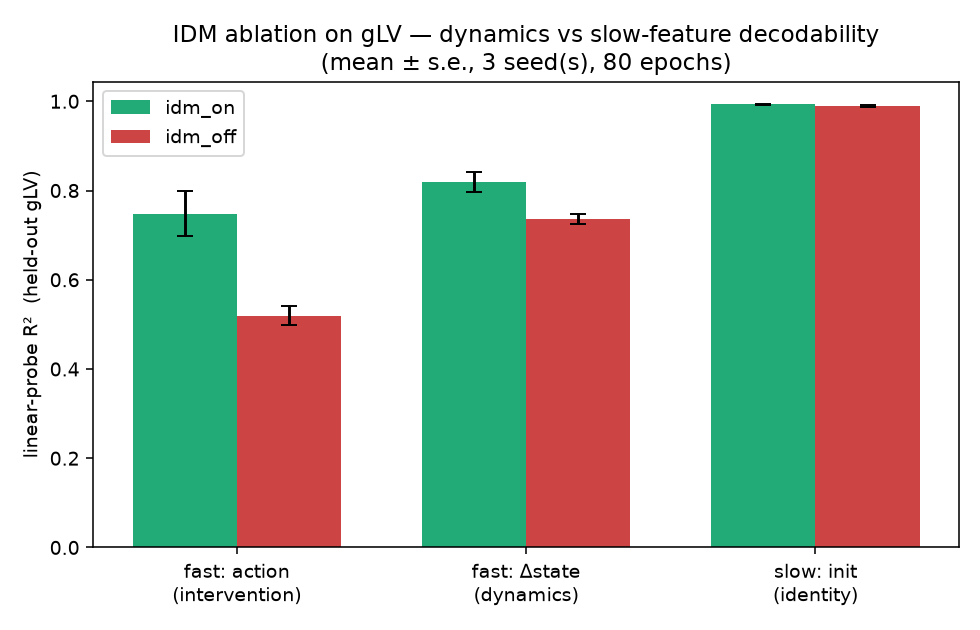
\includegraphics[width=\linewidth]{ablation_collapse.png}
\end{minipage}\hfill
\begin{minipage}{0.49\textwidth}\centering
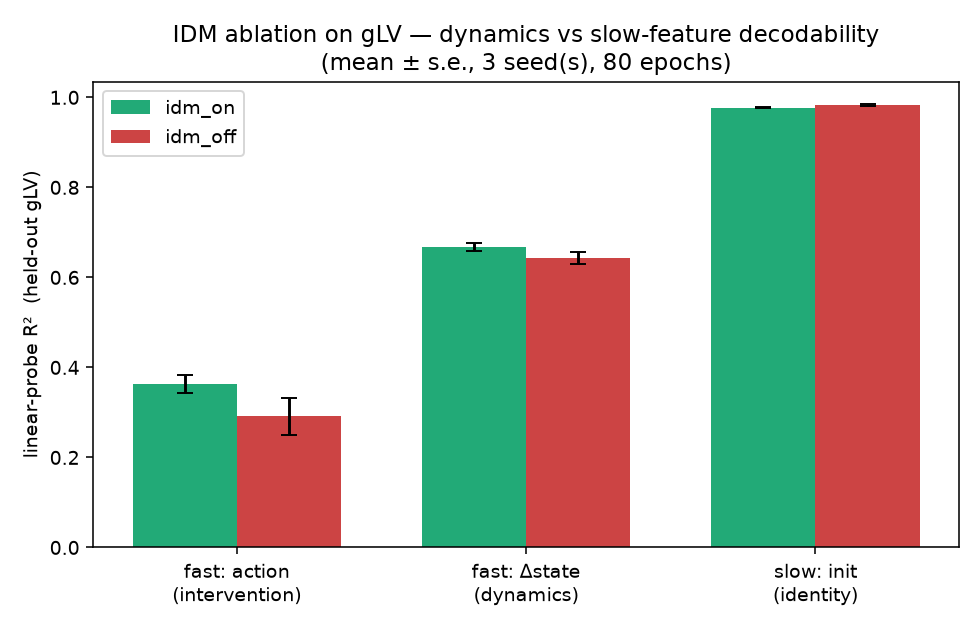
\includegraphics[width=\linewidth]{ablation_default.png}
\end{minipage}
\caption{IDM ablation. \textbf{Left:} induce-collapse regime --- IDM (green)
strongly recovers action decodability over no-IDM (red); identity is saturated.
\textbf{Right:} strong-VICReg default --- the gap is small and overlaps. The IDM
effect is regime-dependent.}
\label{fig:idm}
\end{figure}

\subsection{Short-horizon forecasting: MDSINE2-style benchmark}
\label{sec:benchmark}
On a hold-one-subject-out temporal benchmark (CLR-RMSE at horizons
$h\in\{1,3,5,10\}$, 3 seeds), the JEPA world model is the strongest forecaster
at every horizon, beating persistence, a Ridge gLV-$\ell_2$ baseline, and a
strong gLV-net MLP (Fig.~\ref{fig:benchmark}). This establishes that the latent
predictor is genuinely \emph{faithful} for short-horizon prediction --- a fact
that makes the planning failure in Section~\ref{sec:planning} all the more
striking. (Code and measured JSON: \code{examples/microbiome\_benchmark/}.)

\begin{figure}[h]
\centering
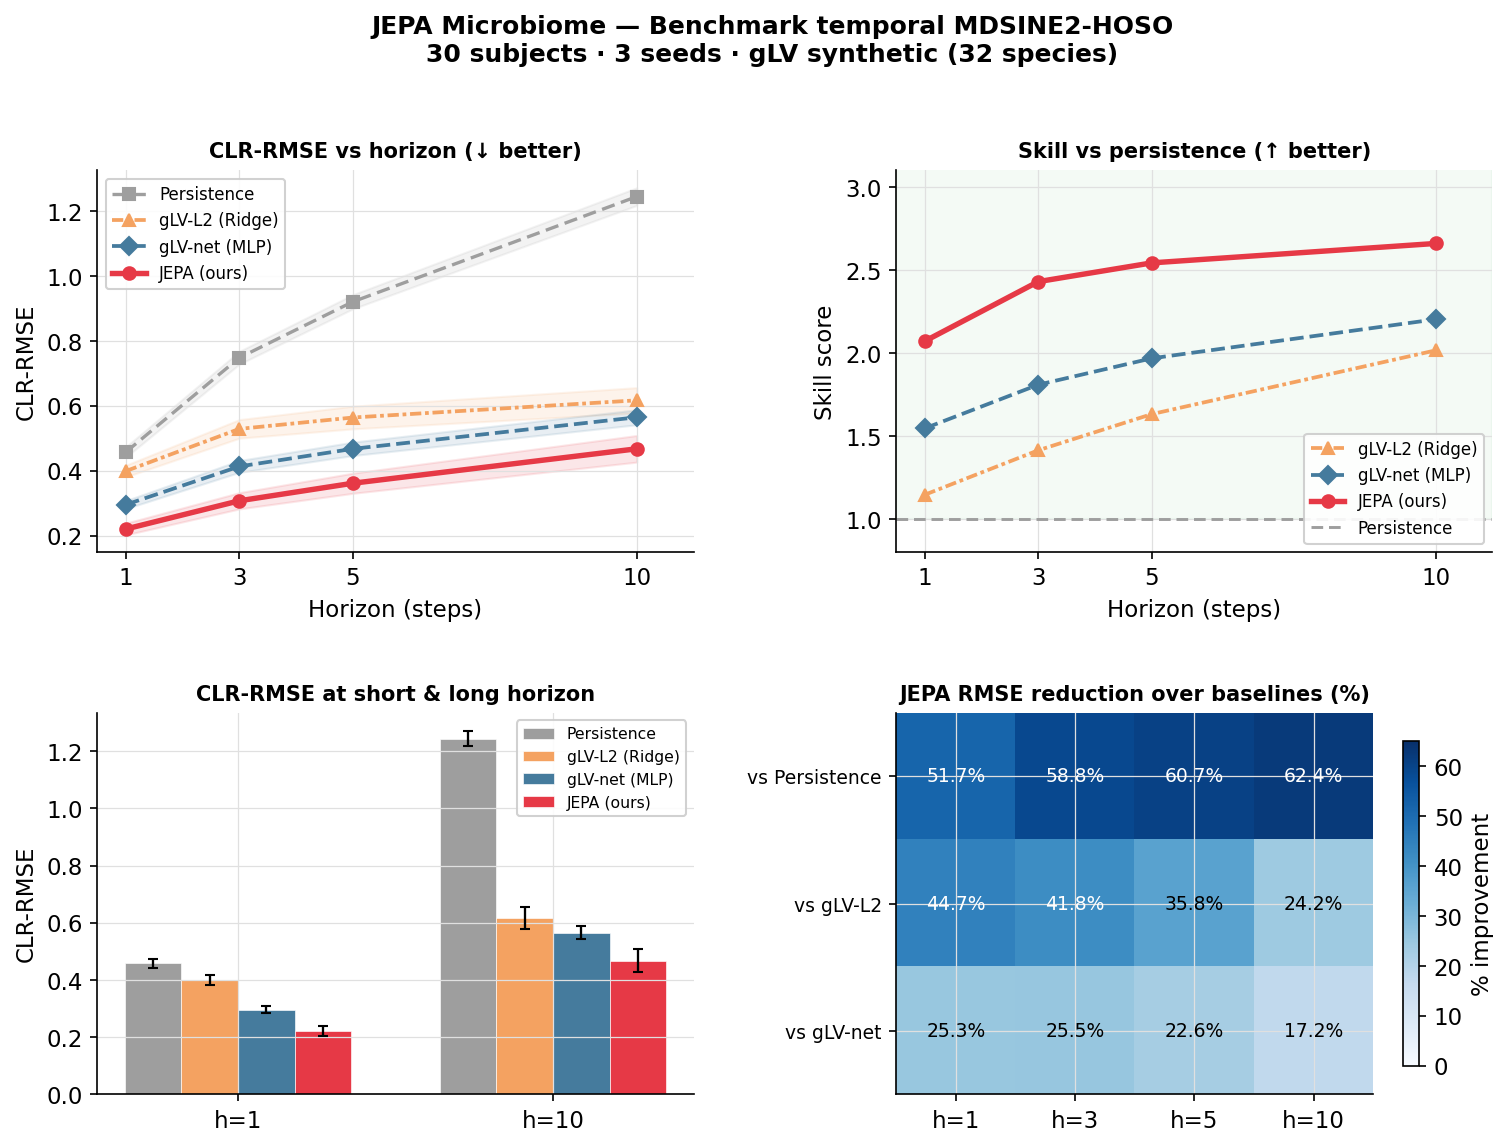
\includegraphics[width=0.86\textwidth]{glv_benchmark_jepa_dashboard.png}
\caption{MDSINE2-style hold-one-subject-out benchmark: JEPA world model vs.\
persistence / gLV-$\ell_2$ / gLV-net across horizons. \meas}
\label{fig:benchmark}
\end{figure}

\subsection{Real-data downstream probe and the SIGReg/VICReg trade-off}
\label{sec:sigreg}
We pretrain a static set-JEPA on a real microbial corpus and probe the frozen
embedding on the Susagi infant-environment task with an apples-to-apples MLP
probe and a corpus z-score. \meas: a SIGReg (LeJEPA) encoder at $d{=}256$
matches the published baseline ($0.5255/0.8936$ vs.\ $0.5270/0.8898$
accuracy/AUC), and at $d{=}384$ beats it on both axes ($0.5309/0.8986$); a
fine-tuned upper bound ($0.5899/0.9180$) exceeds the published reference. A fair
VICReg-$d128$ run sits just below baseline ($0.4995/0.8884$), and an EMA teacher
consistently \emph{hurts} ($0.526\!\rightarrow\!0.507$ MLP).

Critically, the regularizer that \emph{wins} the frozen-probe task is the
\emph{wrong} choice for planning. Replacing VICReg with SIGReg on the planning
world model makes the embedding isotropic ($\code{feat\_std}~0.01\!\rightarrow\!0.50$)
but drives the latent-vs-true distance correlation \emph{negative}
(Pearson $-0.23$) and inflates rollout error --- isotropy is not the same as a
plannable metric. This tension (isotropy helps probing, hurts planning)
motivates the diagnosis below.

\subsection{Planning: a diagnosed negative and its closure}
\label{sec:planning}
This is the core of the paper. The task: steer the simulated community from one
attractor to another, crossing a tolerance set at $15\%$ of the inter-attractor
distance.

\paragraph{(a) The task is solvable (oracle controllability, \meas).}
MPPI on the \emph{true} gLV state reaches $100\%$ success with final distance
$0.790$ when all $K{=}24$ species are actionable, and $0\%$ for $K\le21$
(Fig.~\ref{fig:oracle}). Controllability is a property of the action budget, and
the budget is adequate --- so any downstream failure is the model's, not the
task's.

\paragraph{(b) Pure-JEPA latent MPPI fails completely (\meas).}
Planning with the learned latent cost succeeds $0\%$ of the time. The latent
cost is \emph{uninformative}: its rank correlation with true distance-to-target
is Pearson $-0.002$, Spearman $+0.02$ --- essentially noise --- even though the
\emph{rollout} is faithful ($\approx2\%$ one-step error). Faithful prediction,
useless metric.

\paragraph{(c) Readout fidelity is not the bottleneck (\meas).}
Planning in a \emph{decoded} state space improves with decoder quality: across
two decoder settings (default-regularized, $R^2\!\approx\!0.78$, decoded-MPPI
final $4.12$; weakly-regularized, $R^2\!\approx\!0.89$, final $3.01$), the
stronger decoder's final distance beats a greedy baseline ($3.26$), yet planning
\emph{never crosses tolerance}. Better readout buys a better final distance, not
success.

\paragraph{(d) Eight levers, still $0\%$ (\meas).}
We attack the failure from every side and each is a clean negative: a learned
monotonic cost head (rank correlation $0.71\!\rightarrow\!0.81$ with capacity,
planning flat); an ensemble epistemic gate (uniform disagreement, not
exploitable); on-policy (DAgger/MBPO-style) retraining (planner-trajectory error
falls to $\approx0.135$, planning still $0\%$, final worsens); a multi-step
free-running rollout objective (6-step error cut $0.611\!\rightarrow\!0.086$,
$-86\%$, planning still $0\%$). Dynamics fidelity is \emph{exonerated}; the
bottleneck is the geometry of the representation, not the predictor
(Fig.~\ref{fig:diagnosis}).

\begin{figure}[h]
\centering
\begin{minipage}{0.46\textwidth}\centering
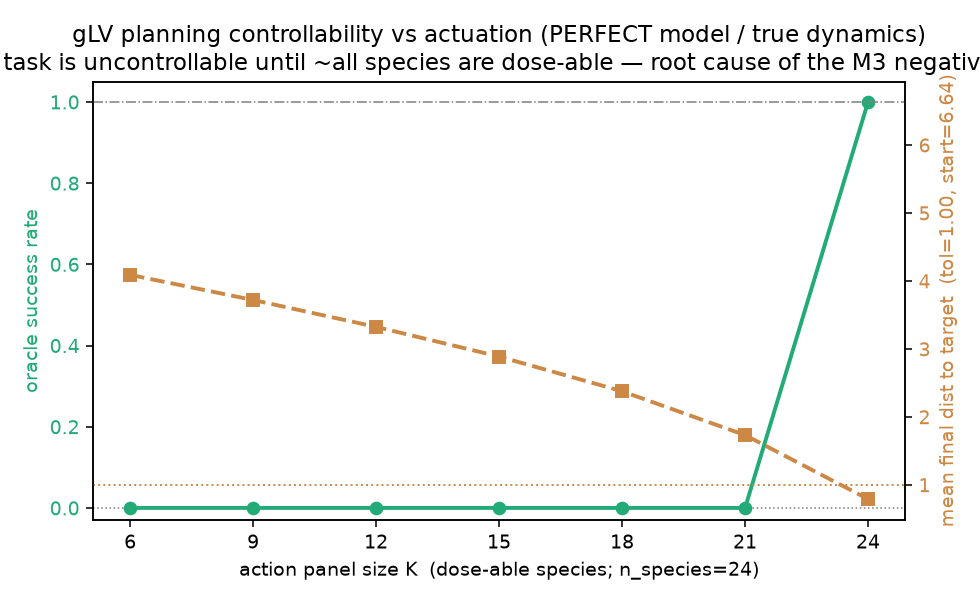
\includegraphics[width=\linewidth]{oracle_K_sweep.png}
\caption{Oracle controllability vs.\ action budget $K$: $100\%$ at $K{=}24$,
$0\%$ for $K\le21$. \meas}
\label{fig:oracle}
\end{minipage}\hfill
\begin{minipage}{0.50\textwidth}\centering
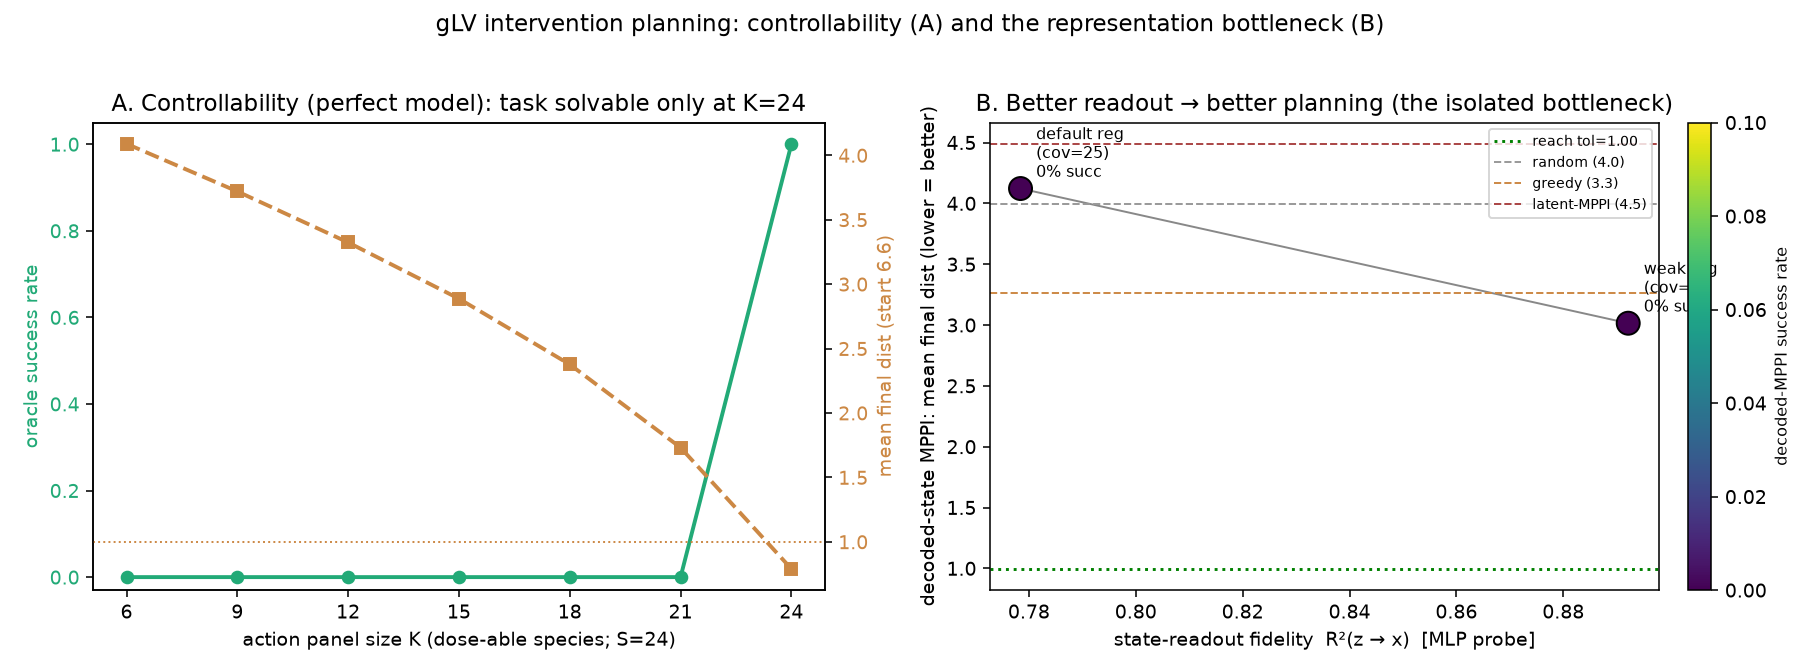
\includegraphics[width=\linewidth]{planning_diagnosis.png}
\caption{Layered diagnosis: controllable task $+$ faithful rollout $+$
\emph{uninformative latent cost} $\Rightarrow$ representation geometry is the
bottleneck. \meas}
\label{fig:diagnosis}
\end{minipage}
\end{figure}

\paragraph{(e) Closing the loop: the metric auxiliary (\meas).}
Adding the isometry auxiliary of Section~\ref{sec:planning-method} (HYBRID,
$\code{metric\_coeff}{=}0.3$) turns raw-latent MPPI from $0\%$ to
$\mathbf{100\%\pm0\%}$, with final distance $0.804$ --- statistically
indistinguishable from the oracle's $0.790$ --- while the latent-vs-true rank
correlation jumps from $0.085$ to $\mathbf{0.990}$ (Fig.~\ref{fig:hybrid}). A
sweep of \code{metric\_coeff} shows a graceful trade-off: success erodes
$100\!\rightarrow\!97\!\rightarrow\!92\%$ as the metric weight grows and the
free-running rollout error rises, with $0.3$ the sweet spot; community
``recognition'' (dominant-guild and basin identification) also improves. We are
explicit that this is a \emph{hybrid}, not a pure JEPA result: the auxiliary uses
true gLV-state distances as supervision (Section~\ref{sec:integrity}).

\begin{figure}[h]
\centering
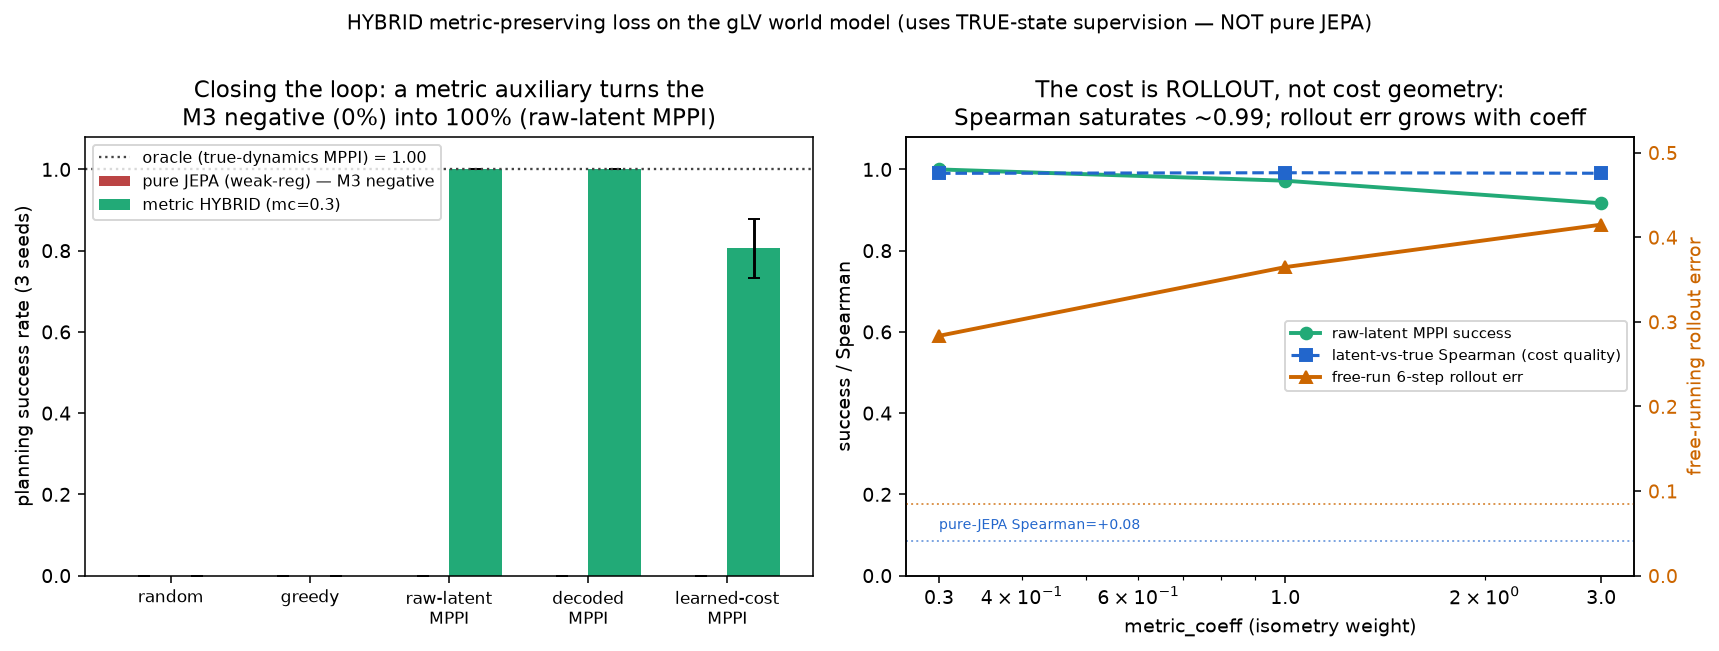
\includegraphics[width=0.72\textwidth]{metric_hybrid.png}
\caption{The isometry auxiliary closes the planning loop: pure JEPA $0\%$ vs.\
HYBRID $100\%$ at oracle quality, with latent$\leftrightarrow$true rank
correlation $0.085\!\rightarrow\!0.990$. \meas}
\label{fig:hybrid}
\end{figure}

\paragraph{(f) Generalization and falsification (\meas).}
The closure is not instance-specific: HYBRID at $\code{metric\_coeff}{=}0.3$
crosses tolerance on $4/4$ diverse gLV instances (pure JEPA $0\%$ on all),
matching the oracle ($100\%$) on $2/4$ and reaching $88.9\%\pm7.3$ on the other
two. Two falsifiers confirm the metric must be \emph{supplied}: a purely
self-supervised IDM-reweighting drives the latent$\leftrightarrow$true
correlation \emph{negative} ($+0.085\!\rightarrow\!-0.313$) and never plans;
shrinking the bottleneck toward the true-state dimension nudges the correlation
only marginally ($\approx0.2$) and costs recognition --- again $0\%$. A
privileged metric is necessary and is not coercible from self-supervision alone
on this testbed.

\subsection{Sequencing-technology invariance}
\label{sec:tech}
Should a microbiome embedding be invariant to the \emph{sequencing technology}
(amplicon vs.\ whole-genome) that produced it? We first measure a confounding
ceiling: biology partially predicts technology (balanced accuracy
$\approx0.69$), so perfect invariance would cost biology. Counter-intuitively,
the \emph{trained} JEPA is \emph{more} technology-separable than its raw input
(SIGReg $0.967 >$ VICReg $0.952 >$ raw $0.938 >$ random $0.897$). We then test
two removal strategies (Fig.~\ref{fig:tech}). A domain-adversarial head (DANN)
\textbf{fails}: technology accuracy never drops below $0.90$ (never near the
$0.69$ floor) while biology is lost about three times faster. A deterministic
moment-matching alignment (CORAL) gives a \textbf{partial} win: SIGReg+CORAL
removes a linear technology leak ($0.934\!\rightarrow\!0.844$, $-0.090$) at
essentially flat biology ($\approx0.77$), but an MLP probe still recovers
technology at $\approx0.96$ --- the fix is linear-only. Lesson: for a dominant,
largely linear nuisance, \emph{alignment beats adversarial}.

\begin{figure}[h]
\centering
\begin{minipage}{0.49\textwidth}\centering
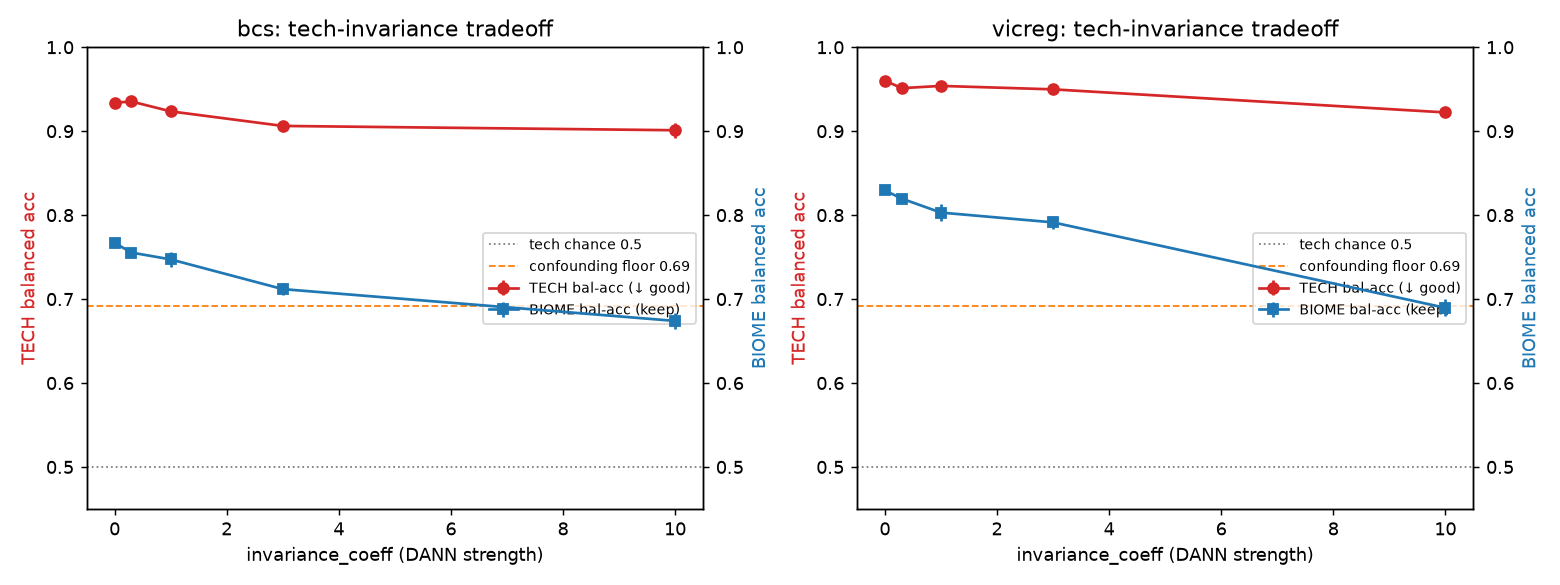
\includegraphics[width=\linewidth]{tech_tradeoff.png}
\end{minipage}\hfill
\begin{minipage}{0.49\textwidth}\centering
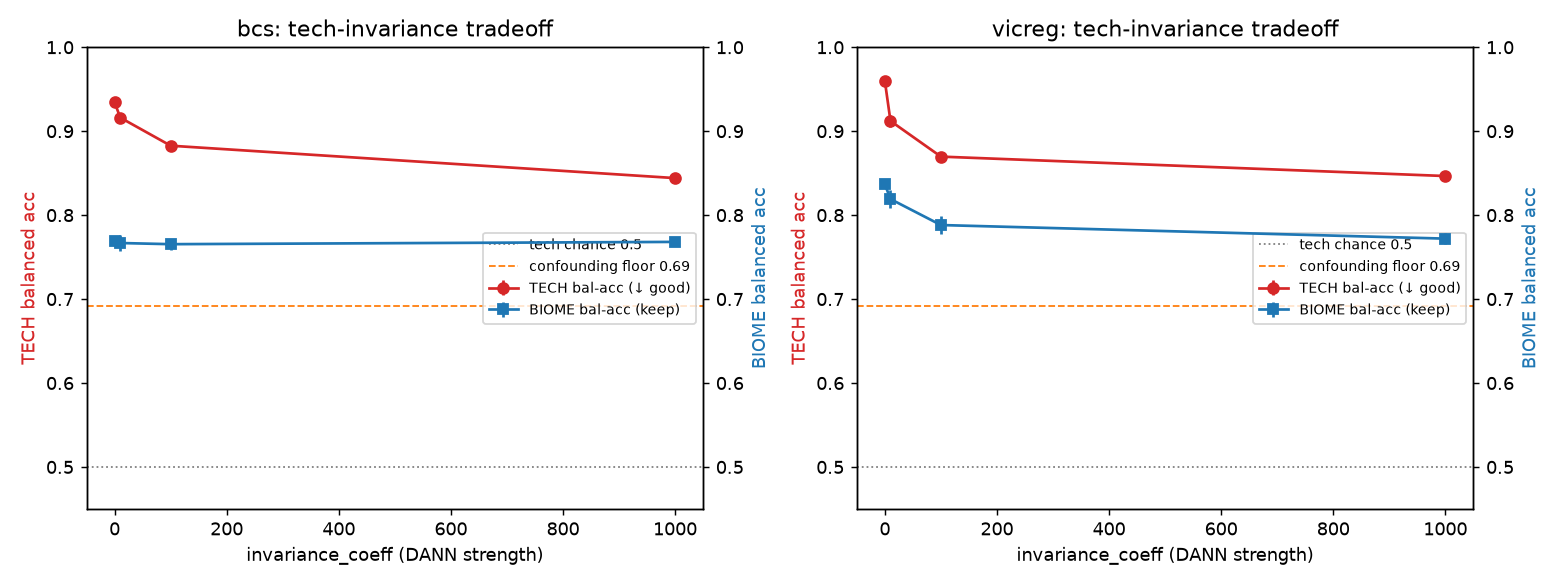
\includegraphics[width=\linewidth]{tech_tradeoff_coral.png}
\end{minipage}
\caption{Technology-vs-biology trade-off. \textbf{Left:} DANN --- biology is lost
$\sim3\times$ faster than technology; no sweet spot. \textbf{Right:} CORAL ---
technology drops while biology stays essentially flat (a clearly favorable
trade), but only the linear leak is removed. \meas}
\label{fig:tech}
\end{figure}

\subsection{Real-world generality: Tahoe-100M drug perturbations}
\label{sec:tahoe}
To test the recipe outside the simulator, we apply the action-conditioned
predictor to real drug perturbations on frozen Tahoe-100M cell-state embeddings
(the encoder is fixed, so there is no collapse to fight). \meas: the predictor
\emph{without} IDM beats a per-drug mean-shift baseline on held-out pairs
($R^2_{\text{shift}}~0.201$ vs.\ $0.149$; the drug is decodable from the true
shift at $75$--$84\%$ top-1, chance $\approx1\%$). Consistent with the
collapse-specific reading of Section~\ref{sec:idm}, IDM here \emph{hurts}
monotonically ($0.201\!\rightarrow\!0.017$). Transfer to unseen cell lines fails
(both arms collapse to around or below a no-op baseline). Single-step action-conditioning partially
generalizes to real data; the IDM auxiliary does not, exactly as the
collapse-specific hypothesis predicts (Fig.~\ref{fig:tahoe}).

\begin{figure}[h]
\centering
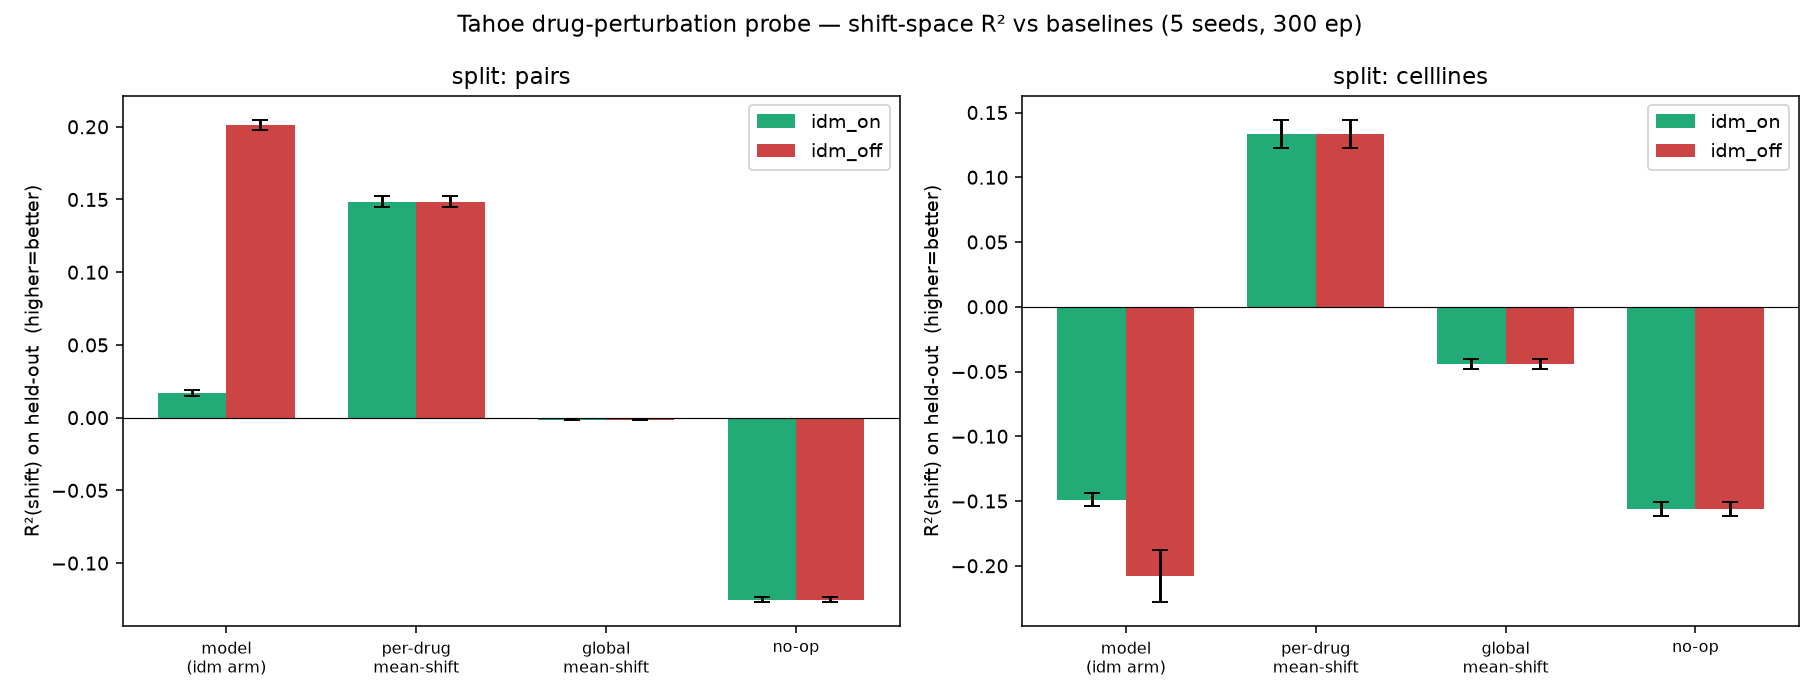
\includegraphics[width=0.72\textwidth]{tahoe_ablation.png}
\caption{Tahoe drug-perturbation probe: the no-IDM predictor beats the per-drug
baseline on held-out pairs (left); cross-cell-line transfer fails (right);
IDM hurts on a frozen encoder. \meas}
\label{fig:tahoe}
\end{figure}

\section{Discussion}
Four lessons cut across the experiments.
\textbf{(1) Faithful prediction is not a plannable metric.} A latent can give
state-of-the-art short-horizon forecasts (Section~\ref{sec:benchmark}) and a
$\approx2\%$ rollout error, yet carry a distance function that is pure noise for
planning. The metric is a separate property and must be earned or supplied.
\textbf{(2) The IDM benefit is collapse-specific.} It rescues fast features when
variance regularization is weak (Section~\ref{sec:idm}) and is redundant ---
even harmful --- on a frozen encoder with no collapse (Section~\ref{sec:tahoe}).
\textbf{(3) Isotropy $\neq$ plannable geometry.} The SIGReg objective that wins
the frozen probe breaks the planning metric (Section~\ref{sec:sigreg}); ``good
for probing'' and ``good for planning'' are different optima.
\textbf{(4) For a dominant linear nuisance, alignment beats adversarial}
(Section~\ref{sec:tech}).

\section{Limitations and integrity}
\label{sec:integrity}
\textbf{The HYBRID is not a pure JEPA.} The planning closure uses true
gLV-state distances as supervision for the isometry term. It demonstrates that
\emph{a} metric closes the loop and that the bottleneck is geometric, but it is
not a claim that pure self-supervision suffices --- indeed our falsifiers show it
does not (Section~\ref{sec:planning}f). \textbf{The unseeded-decoder fluke.} An
early decoded-planning run reported a $2.8\%$ ``success''; we traced it to an
unseeded MLP decoder initialization, seeded it, and the result became a
reproducible $0\%$. The corrected value is the one reported, and the fluke is
recorded in the log rather than quietly dropped. \textbf{Simulator scope.} The
planning results are on a synthetic gLV testbed designed to be controllable and
non-monotonic; the metric closure need not transfer unchanged to real
communities. \textbf{Real-data parsers} for the largest corpus were exercised on
the cluster and are flagged unverified on commodity hardware. \textbf{Provenance
gaps} (e.g.\ one missing baseline JSON, a Tahoe coefficient sweep whose
intermediate log was not committed) are enumerated in \code{docs/WORK\_REPORT.md}.

\section{Conclusion}
Energy-based JEPA world models can encode microbial dynamics well enough to
forecast and, with the right auxiliary, to plan. The decisive insight is that a
faithful predictive latent does not automatically furnish a metric in which
planning works: across eight levers, pure-JEPA latent MPPI never crossed
tolerance, and only an explicit isometry auxiliary --- supplying the missing
geometry --- closed the loop to oracle quality and generalized across instances.
Inverse dynamics rescues fast, action-relevant features precisely when the
representation is collapsing, and not otherwise. We hope the layered, honest
methodology here --- separating controllability, dynamics fidelity, readout, and
metric --- is useful for anyone trying to turn a predictive representation into a
controller.

\paragraph{Acknowledgements / provenance.} This work is built on the
\texttt{eb\_jepa} energy-based JEPA framework
(\url{https://github.com/marinabar/eb_jepa}); the encoder, predictor,
regularizers, and \code{unroll} machinery are upstream and credited under
\code{LICENSE.md}. All experiments, results, and figures reproduced here are the
author's contribution.

\begin{thebibliography}{99}
\bibitem{lecun2022path} Y.~LeCun. \emph{A Path Towards Autonomous Machine
Intelligence}. OpenReview, 2022.
\bibitem{bardes2022vicreg} A.~Bardes, J.~Ponce, Y.~LeCun. \emph{VICReg:
Variance-Invariance-Covariance Regularization for Self-Supervised Learning}.
ICLR, 2022.
\bibitem{sobal2022} V.~Sobal et al. \emph{Joint Embedding Predictive
Architectures Focus on Slow Features}. arXiv:2211.10831, 2022.
\bibitem{lejepa2025} \emph{LeJEPA: Provable and Scalable Self-Supervised
Learning via Sketched Isotropic Gaussian Regularization (SIGReg)}. 2025.
\bibitem{mdsine2} G.~Gibson et al. \emph{MDSINE2: Robust inference of microbial
dynamics from time-series data}. 2021.
\bibitem{williams2017mppi} G.~Williams, A.~Aldrich, E.~Theodorou.
\emph{Model Predictive Path Integral Control}. J.\ Guidance, Control, and
Dynamics, 2017.
\bibitem{ganin2015dann} Y.~Ganin, V.~Lempitsky. \emph{Unsupervised Domain
Adaptation by Backpropagation (DANN)}. ICML, 2015.
\bibitem{sun2016coral} B.~Sun, K.~Saenko. \emph{Deep CORAL: Correlation
Alignment for Deep Domain Adaptation}. ECCV Workshops, 2016.
\bibitem{genejepa2025} Litman et al. \emph{GeneJEPA}. bioRxiv
2025.10.14.682378, 2025.
\end{thebibliography}

\end{document}
